\documentclass[12pt]{article}

\usepackage{times} % times font
\usepackage{setspace} \singlespacing % double space
\usepackage[margin=1in]{geometry} % 1 inch margins
\usepackage{apa} % for bib
\usepackage{graphicx} % for figs

\begin{document}

\section*{Introduction}
This research aims to explore how the brain integrates information from one moment to the next and uses it to drive predictions about what will happen. Our lab has developed a computational model and general framework named LeabraTI (Temporal Integration) that describes this process at the mechanistic level. LeabraTI is closely related to the Simple Recurrent Network (SRN) \cite{Elman90,Servan-SchreiberCleeremansMcClelland91}, a discrete time neural network that learns temporal structure by explicitly representing lagged temporal information in a population of ``context'' units and integrating it with more current information at each time step. LeabraTI provides an explanation of how an SRN-like computation can be realized in a continuous time biological neural network with a number of explicit predictions that can be tested empirically.
	
The central prediction of LeabraTI is that time in the brain is discretized into 100 ms intervals, corresponding to individual cycles of intrinsic alpha-band oscillations. The trough of the alpha cycle indexes a low point of neuronal excitability (\nopcite{KlimeschSausengHanslmayr07}; \abbrevnopcite{MathewsonLlerasBeckEtAl11}), which in the context of LeabraTI, supports generation of an intrinsic prediction about what will happen during the peak of the alpha cycle roughly 50 ms in the future. Learning operates on the differences between neural activations during the trough and the peak to minimize prediction error about incoming sensory information. The peak of the alpha cycle is considerably more excitable than the trough and thus is the optimal time frame of sensory stimulation. A number of studies have noted the importance of alpha-band phase in determining the quality of sensory information \cite{MathewsonGrattonFabianiEtAl09,BuschDuboisVanRullen09,VanRullenBuschDrewesEtAl11}. Furthermore, monkey intracranial recordings suggest that the neural activity can phase-lock to extrinsic rhythmic stimulation (\nopcite{LakatosKarmosMehtaEtAl08}; \nopcite{SchroederLakatos09}), ensuring that stimuli are processed during the high excitability peak of the alpha cycle.

One issue with testing LeabraTI's predictions lays in determining the relationship between prediction and attention. For example, the alpha rhythm might simply correspond to shifts of spatial attention, which can be oriented roughly 10 times per second \cite{VanRullenDubois11}, and studies using a Posner cueing task \cite{Posner80} support this idea \cite[e.g.,]{CapotostoBabiloniRomaniEtAl09,BuschVanRullen10}. Other studies, however, suggest that prediction and attention are  separable mechanisms with dissociable effects \cite{KokRahnevJeheeEtAl12,WyartNobreSummerfield12,ArnalGiraud12,HorschigJensenVanSchouwenburgEtAl13}. Another issue is that LeabraTI predicts that an entire spatiotemporal sequence contributes to the representation of a predicted stimulus in the brain. Many of the tasks used in previous studies of prediction can be performed simply by using information from the time step immediately preceding the stimulus of interest \cite{DohertyRaoMesulamEtAl05,RohenkohlNobre11}, effectively reducing them to a Posner cueing task. These issues are summarized in Figure \ref{fig:previous_expts}.

% previous expos fig
\begin{figure}[h!]
\begin{tabular}{ll}
\textbf{A} & \textbf{B} \\
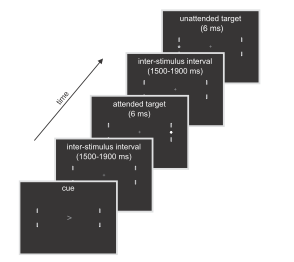
\includegraphics[width=3.5in]{BuschVanRullen10.png} &
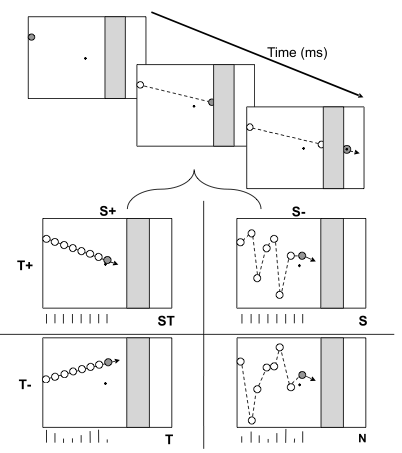
\includegraphics[width=3in]{DohertyRaoMesulamEtAl05.png} \\
\end{tabular}
\caption{\small{Previous investigations of the effect of predictability on alpha-band activity. \textbf{A:} \protect\incite{BuschVanRullen10} used a Posner cueing task to determine the effect of target location predictability on alpha-band activity. However, the effects of prediction in this task are confounded with spatial attention. \textbf{B:} \protect\incite{DohertyRaoMesulamEtAl05} created spatiotemporal sequences of stimuli that reliably and unreliably predicted location and temporal onset of a target. However, the task can be performed by simply using information from the time step preceding the target (in this case, before the ball travels behind the gray occluding band), effectively reducing it to a Posner cueing task.}
\label{fig:previous_expts}}
\end{figure}

\section*{Proposed research}
To address the issues raised in the previous section, the proposed research will use a task devoid of spatial attention orienting. The basic paradigm is depicted in Figure \ref{fig:proposed_expt}. Novel three-dimensional stimuli will be presented at the center of a display and rotated about their axes while subjects maintain fixation. The temporal order of the presentation frames can be varied to manipulate the frame-to-frame predictability and the onset of each frame can be adjusted to be in-phase or out-of-phase with a 10 Hz presentation rate. Both of these factors will be controlled independently. After viewing each frame sequence, subjects will perform a same/different judgement about a probe stimulus.

% proposed expt fig
\begin{figure}[h!]
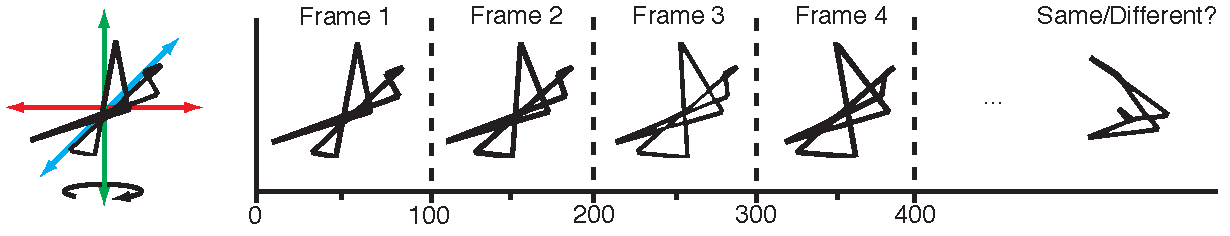
\includegraphics[width=6.5in]{Paperclip.pdf}
\caption{\small{Basic experimental paradigm. Novel three-dimensional objects will be given coherent motion (e.g., rotating about their y-axis)} and presented either in-sequence or in random order and the temporal onset of each frame will be adjusted to be in-phase or out-of-phase with a 10 Hz presentation rate. After viewing the frame sequence, subjects will perform a same/different judgement about a probe stimulus.}
\label{fig:proposed_expt}
\end{figure}

It is important to use novel objects to ensure that subjects do not have prior familiarity with their three-dimensional structure. Wireframe ``paperclip'' objects provide a reasonable solution to this problem and have the additional benefit of being parametrically controllable for similarity (e.g., Euclidean distance between pairs of vertices from two objects). These objects have also been used in a variety of models and studies on object recognition and view invariance \cite[e.g.,]{PoggioEdelman90,BulthoffEdelman92,EdelmanBulthoff92,LogothetisPaulsBulthoffEtAl94,LogothetisPaulsPoggio95,RiesenhuberPoggio99,BalasSinha09b}, making it easy to relate results to previous efforts.

EEG will be recorded and analyzed for ERP differences between conditions as well as their dependency on alpha phase at probe onset. LeabraTI predicts that frames presented in-sequence will maximize sensitivity for same/different judgements, especially when frames are in-phase with a 10 Hz presentation rate due to build-up of a robust object representation. Out-of-phase presentation is likely to impair discrimination to some extent, but possibly only for judgements that are highly ambiguous (e.g., low contrast or perceptually similar probes). These effects will be characterized by calculating instantaneous phase, power, and related measures
\footnote{Inter-trial coherence \cite{Tallon-BaudryBertrandDelpuechEtAl96}}$^,$
\footnote{Phase-locking value \cite{LachauxRodriguezMartinerieEtAl99,SchackKlimesch02}}$^,$
\footnote{Phase-preservation index \cite{MazaheriJensen06}} 
over the full course of frame sequence to infer the quality of the object representation. Initial data from a similar experimental task \cite{DohertyRaoMesulamEtAl05} suggests that there are differences in this build-up that could contribute to recognition success at probe onset (Figure \ref{fig:pilot_expt}).

% pilot expt fig
\begin{figure}[h!]
\centering
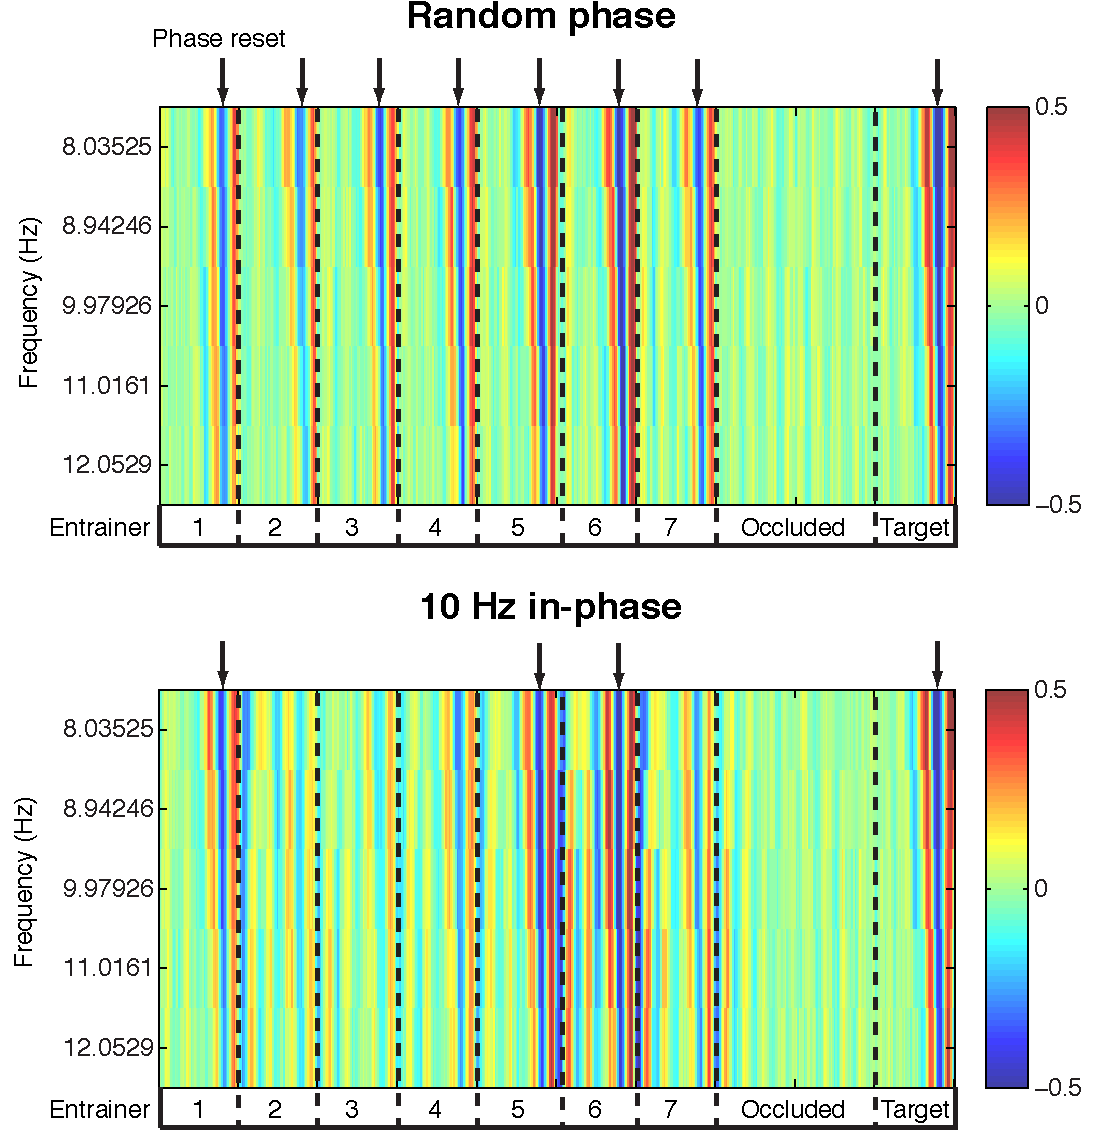
\includegraphics[width=5.5in]{phase_OBI.pdf}
\caption{\small{EEG phase-locking to temporally predictable stimulation}. A paradigm similar to \protect\incite{DohertyRaoMesulamEtAl05} in which an entraining stimulus travels across the screen in either a temporally unpredictable manner (top) or in-phase with a 10 Hz presentation rate (bottom) before disappearing behind an occluding band and reappearing with a target. Instantaneous phase in the alpha-band spectrum is depicted for a bilateral pool of posterior electrodes. Phase resetting can be observed for each individual stimulus in the random case consistent with the brain's alpha rhythm attempting to synchronize with an unpredictable presentation rate. Less phase resetting is present for the 10 Hz case indicating successful synchronization with the predictable presentation rate. Data depicted are averaged over eight subjects.}
\label{fig:pilot_expt}
\end{figure}

% other exps
%
% attn/relevance/oddball
% # of entrainers
% diff stimulation freqs
% masking
% training

The basic experimental paradigm will be built upon by a follow-up experiment that investigates a related question such as:
\begin{enumerate}
\item How much temporally predictable entrainment is necessary to build a robust object representation? \incite{MathewsonFabianiGrattonEtAl10} shows that the effects of metacontrast masking can be abolished with as few as two entraining stimuli that establish a rhythmic sequence, but effect sizes increase with additional entraining stimuli. Furthermore, how do these effects interact with frame-to-frame predictability?
\item What is interaction between stimulus ambiguity and temporal predictability. Can relatively coarse perceptual judgements be made without temporal predictability? Are there differences when a ``same'' probe is a view presented during the entraining sequence versus a novel view (i.e., view generalization).
\item What is the role of presentation rate when stimuli are temporally predictable? LeabraTI suggests that 10 Hz is an optimal rate for ensuring that prediction and sensation can operate in synchrony with thalamocortical loops. However, some experiments observe effects that are dependent on presentation rate outside the alpha-band such as an inversion effect at 15 Hz but not 30 Hz (\nopcite{BalasSinha09}; see also \abbrevnopcite{deGraafGrossPatersonEtAl13}; \nopcite{SchultzBrockhausBulthoffEtAl13}).
\end{enumerate}

In addition to two EEG experiments, simulations using the LeabraTI framework will be used to model the behavioral effects and determine mechanistically what is driving them. For example, it might be the case that sequences presented in random order generate an effect similar to masking in which top-down predictions are inconsistent with bottom-up sensory information, leading to a poor quality object representation. Temporal unpredictability could have a similar effect, but due to inconsistencies in the amount of time the brain requires to generate a prediction or properly process sensory information.

\bibliographystyle{apa}
\bibliography{ccnlab}
\end{document}